% !TEX root = ../main.tex
\documentclass[../main.tex]{subfiles}
\begin{document}
\label{sec:results}

In this Section we explore the consistency with which volunteers modelled galaxies, the variance of the aggregate model recovered and compare our recovered models to other results in the literature.

\subsection{Examination of Volunteer consistency}
We aggregate two independent models for a set of 98 galaxies based on ``original'' or repeat (``validation'') classifications, obtained with the same retirement limit (see Section \ref{sec:retirement-limit} for more on this selection).

One of the simplest choices the volunteers have is whether to include a model component or not. Figure \ref{fig:volunteer_component_consistency} illustrates the consistency with which volunteers made use of a component in their model for a galaxy. We see that volunteer classification is very consistent (scatter in fraction of 0.1), with volunteers almost always using a disc and bulge, and consistent proportions agreeing on the presence of a bar and the number of spiral arms.

\begin{figure*}
  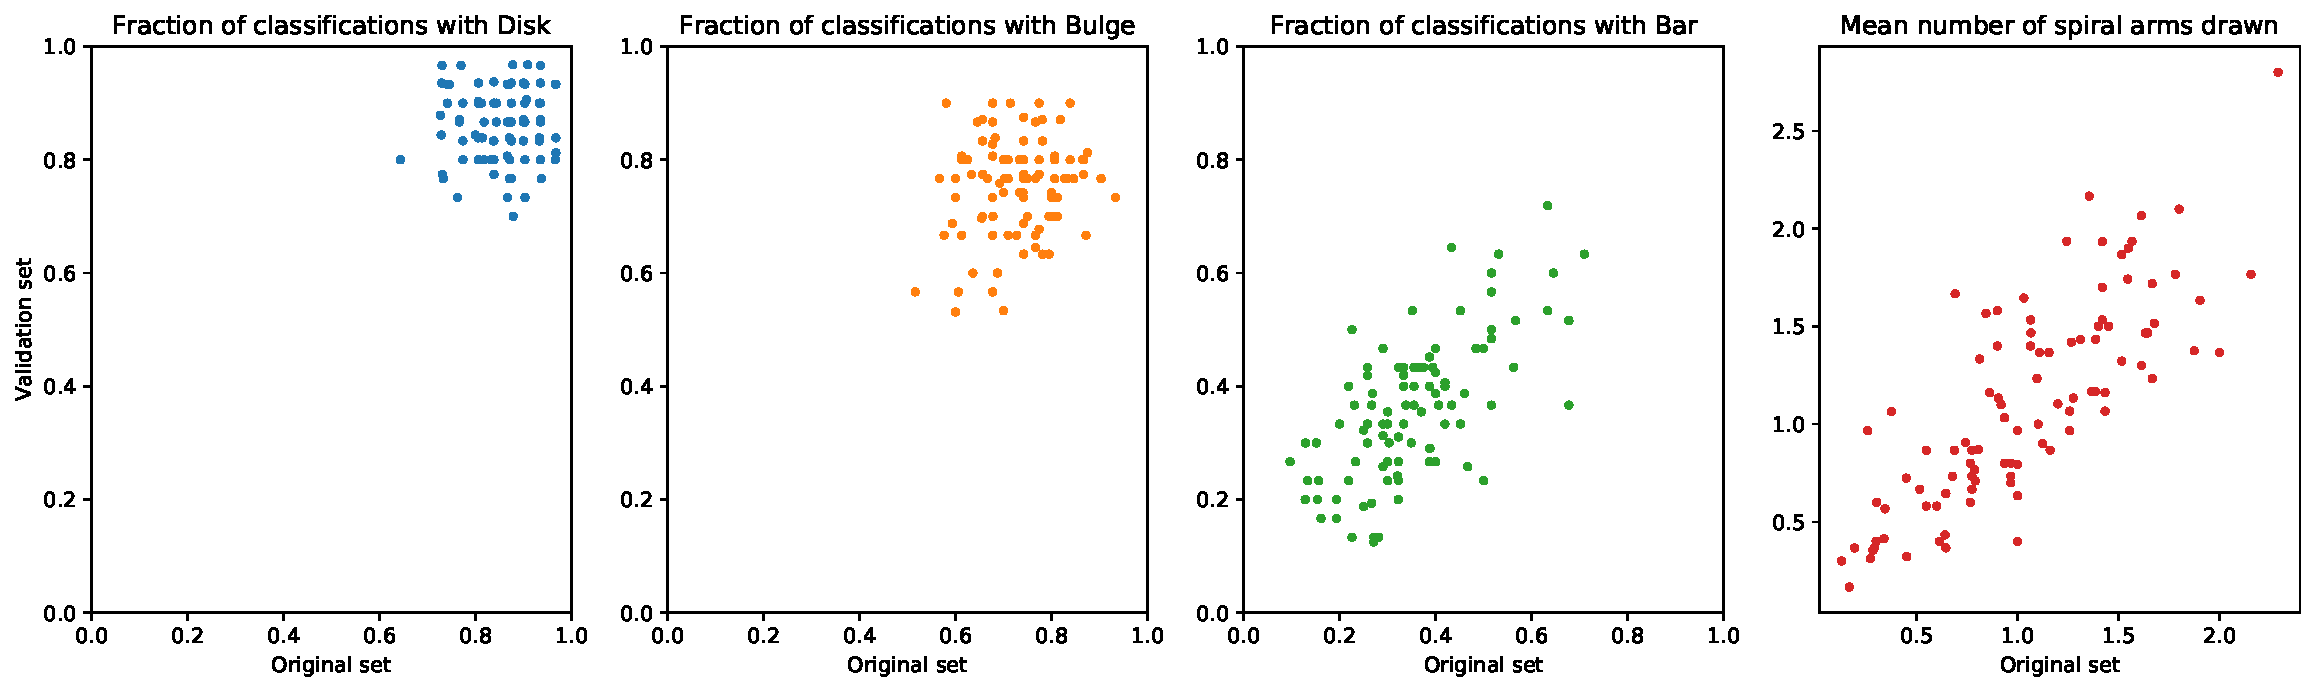
\includegraphics[width=17.3cm]{images__results/component_frequency.pdf}
  \caption{Comparison of frequency of use of component in volunteer models between the original and validation sets of classifications.}
  \label{fig:volunteer_component_consistency}
\end{figure*}

After selecting a component, the volunteer sets its shape and size. We see generally good consistency in isophotal shape and size, with the least consistent component is the bar, which may be caused by the lower proportion of volunteers incorporating one into their model. Visual inspection suggests that many volunteers used a very elliptical bulge and drawn spirals to capture the light from the bar. Fewer bars having been drawn by volunteers also has the effect of making clustering more difficult and more uncertain, even for a strongly barred galaxy we effectively go from receiving 30 classifications to around 12 for the bar. The variation in axial ratios and effective radii for the aggregate discs, bulges and bars are shown in Figure \ref{fig:aggregate_model_consistency}: the sample error in disc size is 3.8 arcseconds, bulge size is 1.6 arcseconds and bar size is 1.5 arcseconds. There is very little consistency in axial ratio for the bulge and bar, however the disc axial ratio shows good consistency, with a sample error of 0.064.

\begin{figure*}
  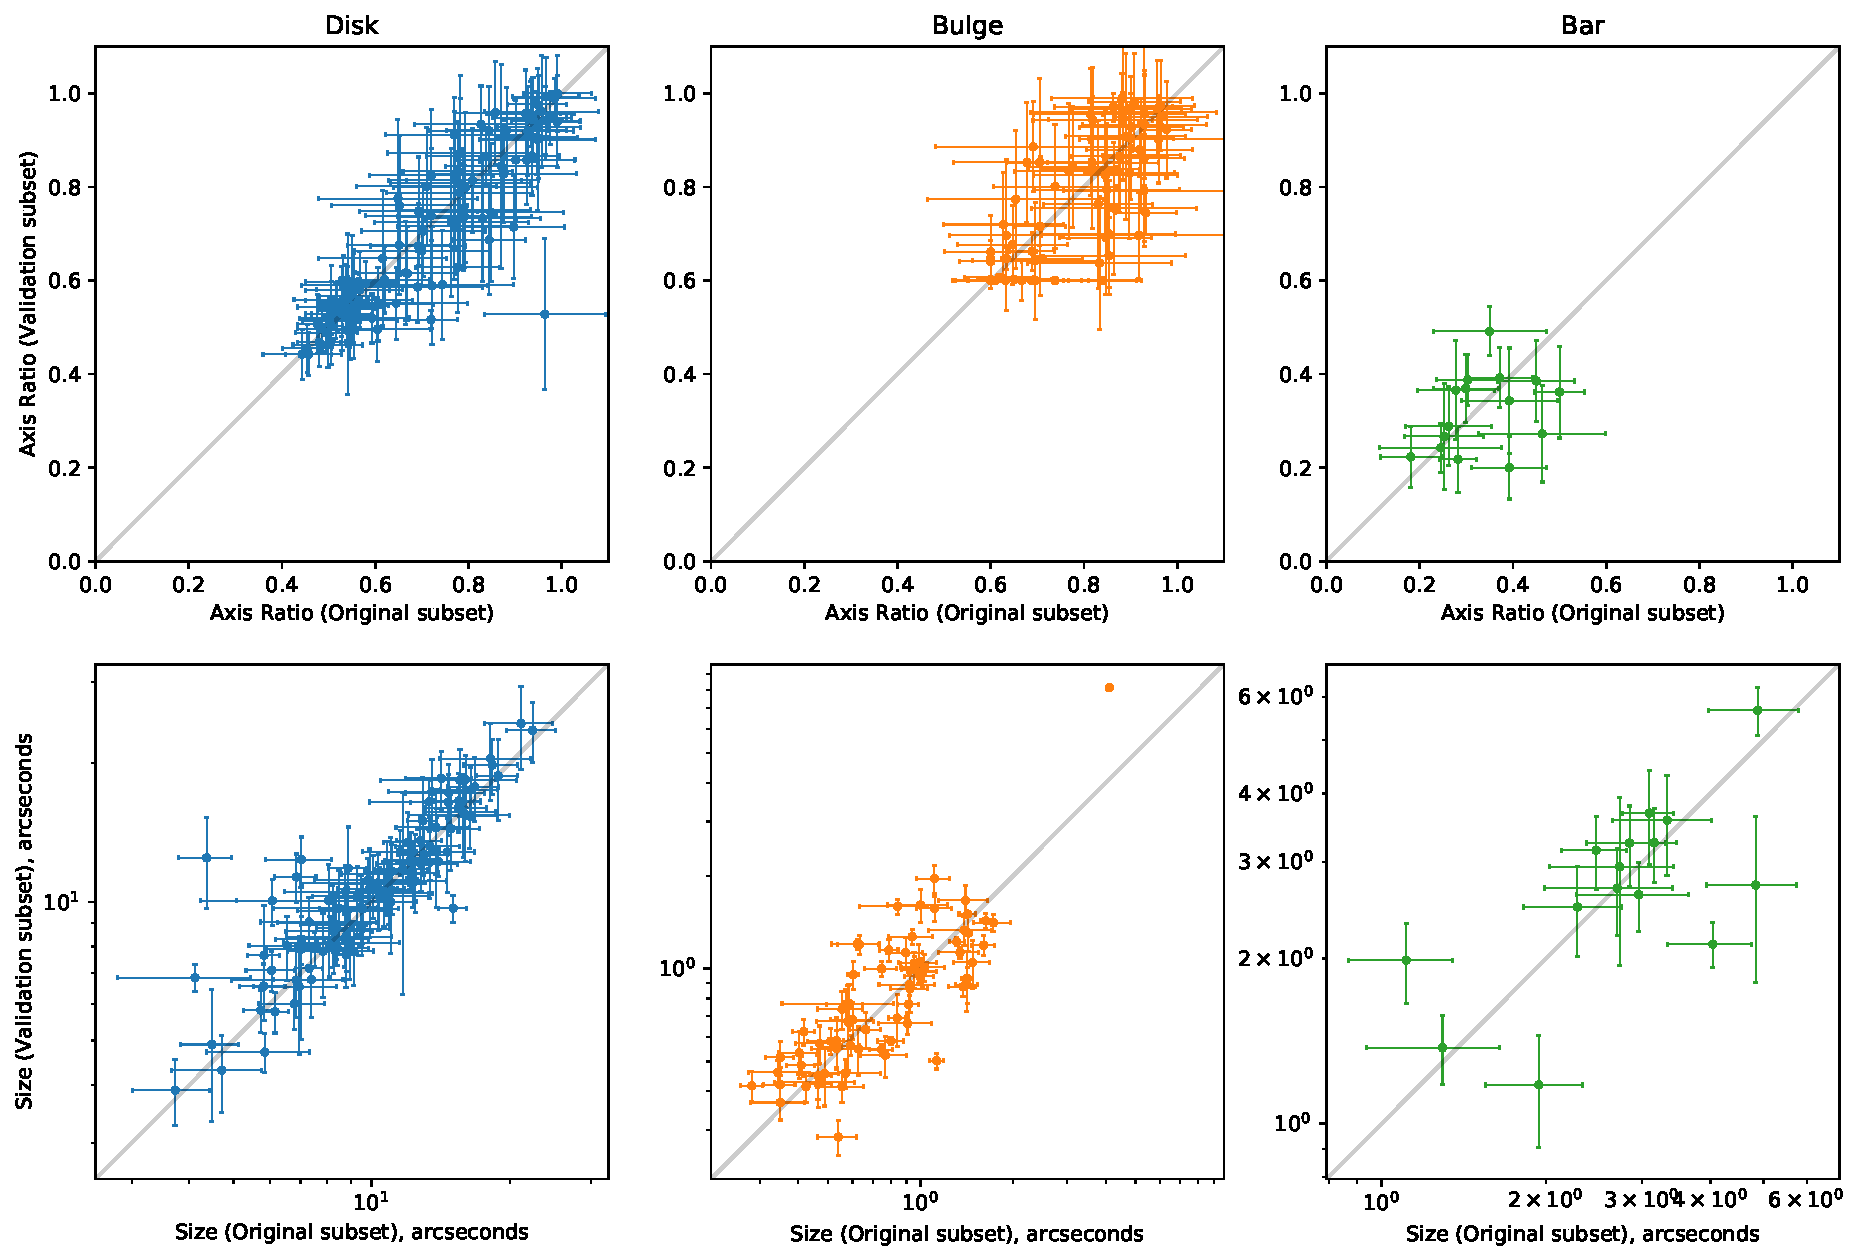
\includegraphics[width=17.3cm]{images__results/component_sizing.pdf}
  \caption{Comparison of component shape in aggregate models between the original and validation sets.}
  \label{fig:aggregate_model_consistency}
\end{figure*}

\subsection{Comparison to results in the literature}

\comment{REDO THIS WHOLE SECTION}

After having obtained aggregated models for our galaxies, we examine how our models compare to other results in the literature. There exists no published comparison sample with four-component fits, instead we make comparisons for individual or subsets of model components.

\subsubsection{Comparison to Galaxy Zoo morpohology}

When comparing the probability of a volunteer's classification containing a bar component against a galaxy being classed as strongly-barred or as having no bar (as defined in \citealt{Masters2010:1003.0449v2}), we see a significant difference: classifications of strongly-barred galaxies ($p_\text{bar} > 0.5$) had a $0.47 \pm 0.14$ chance of containing a bar, vs $0.30 \pm 0.11$ for galaxies classed as having no bar ($p_\text{bar} < 0.2$). The Spearman correlation between GZ2's $p_\text{bar}$ and the bar likelihood in \textit{Galaxy Builder} is $0.56$, implying a significant correlation.


\subsubsection{Comparison to One-component fit - axis ratio}
We compare the axis ratios of the discs of \textit{Galaxy Builder} aggregate models (without tuning) to the axis ratio of a 2D S\'ersic fit to the r-band SDSS image of each galaxy (as provided in the NSA catalog, \citealt{2011AJ....142...31B}).

We see excellent agreement for all types of \textit{Galaxy Builder} models (Figure \ref{fig:ax_ratio_comparison}). For the untuned models there is an error of $\sim0.1$, consistent with our expected errors (derived in Section \ref{sec:error_estimation}). For the aggregate model, 23\% measurements with axis ratio less than 0.6 are outside $2\sigma$, significantly higher than the expected 5\%. This is opposed to 5.0\% of measurements with axis ratio greater than 0.6. There is a clustering of outlying values at $b/a=0.5$ which is almost certainly due to the drawing tool ellipse having a default axis ratio of 0.5. Where this default is a ``good enough'' fit we hypothesise that volunteers are less likely to modify it, while if it needs to move a long way they find a more refined value. We see similar behaviour in the cluster of values at $b/a=1$ representing volunteers hitting the maximum value and not refining further.

Volunteers not adjusting components from their default values was a consistent issue with untuned models (36\% of all disc components drawn by volunteers were left at the default axis ratio, and over half of all bars were left with their default rotation, though many of these would have been excluded during clustering). Future projects should carefully consider their interface design to minimize this bias. Fitting aggregate models successfully removes this bias, and reduces the error between \textit{Galaxy Builder} disk axis ratios and that of the NSA S\'ersic fit to \comment{$0.07$}.

\begin{figure}
  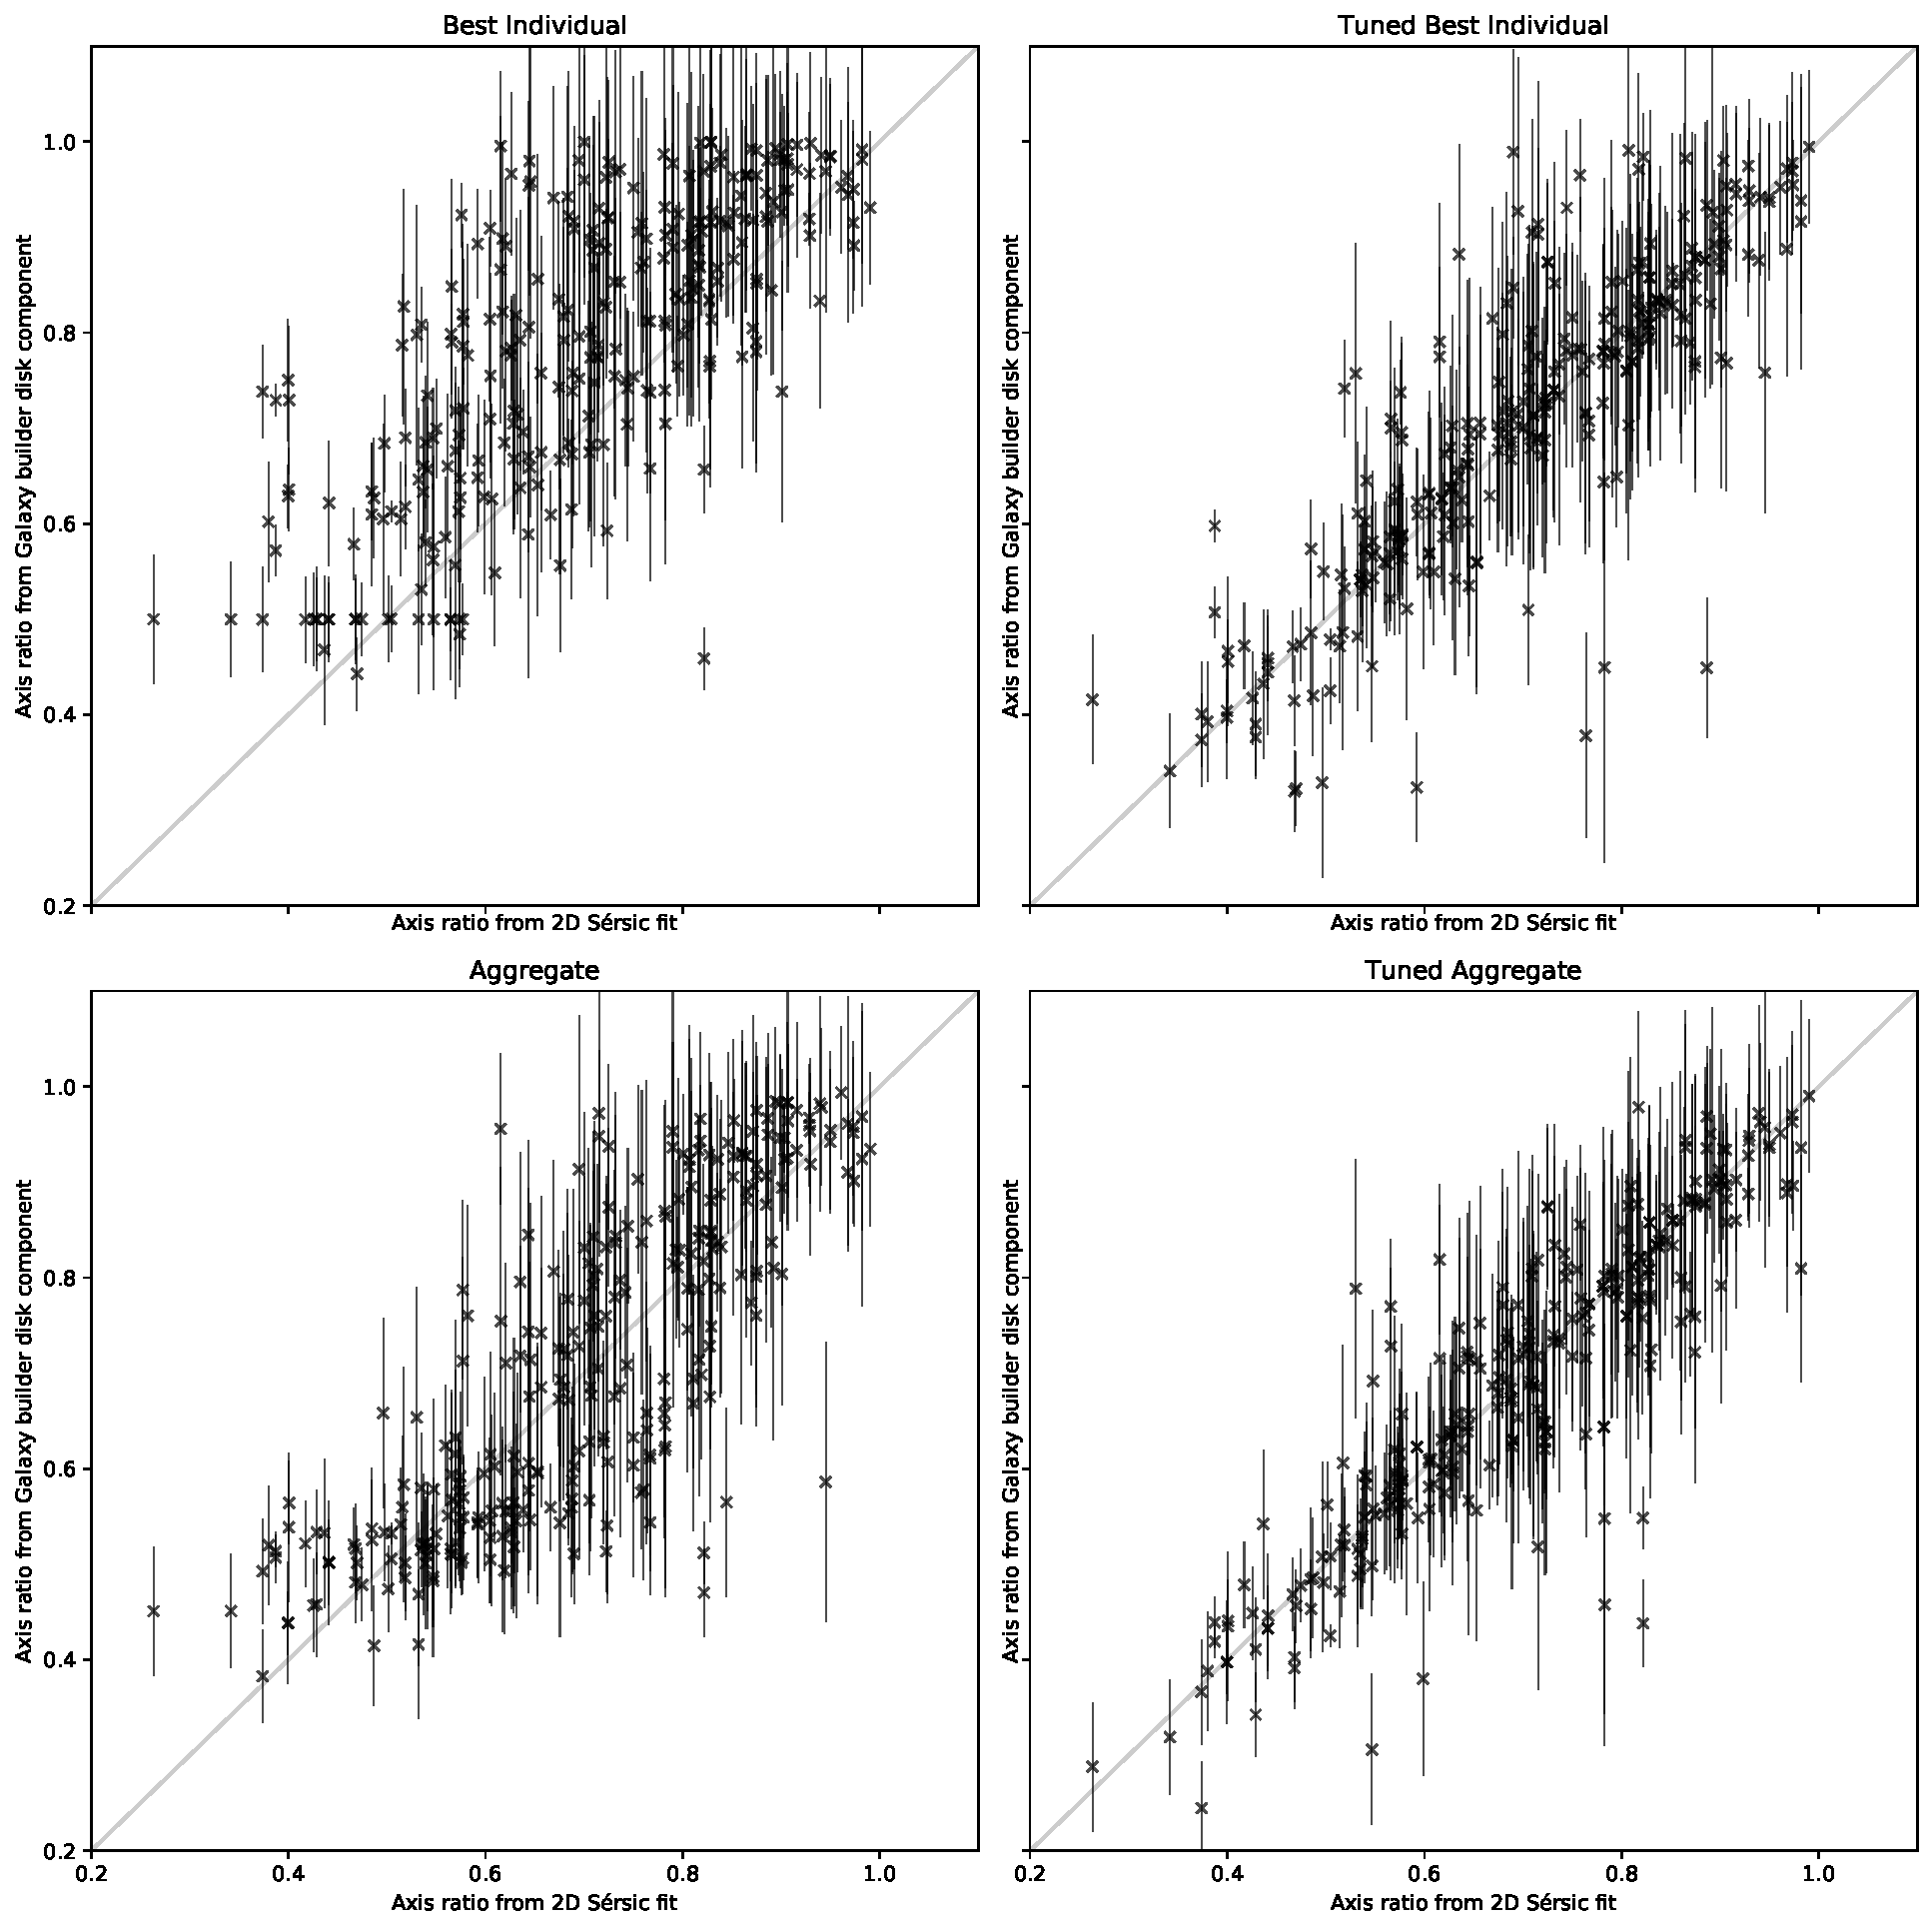
\includegraphics[width=8cm]{images__results/gzb-agg-nsa-comparison_all.pdf}
  \caption{Difference between the axis ratios of the disc components of various \textit{Galaxy Builder} models to the results of an r-band S\'ersic profile fit.}
  \label{fig:ax_ratio_comparison}
\end{figure}


\subsubsection{Comparison to Disc-Bulge models}

One of the largest catalogs of 2D multi-component fits is \citet{2011ApJS..196...11S}, which performed simultaneous, two-bandpass decompositions of 1,123,718 galaxies in the Legacy area of the SDSS DR7 using \textsc{Gim2D}. Three variations of models were fitted: a pure S\'ersic model, an exponential disc and de-Vaucouleurs bulge model, and an exponential disc and a S\'ersic bulge model. \citet{2012MNRAS.421.2277L} similarly fitted two models to SDSS main-sample galaxies: an exponential disc and exponential bulge (exp+exp), and an exponential disc and de Vaucouleurs bulge (exp+dV). They used a Levenberg-Marquadt gradient descent algorithm, with initial parameters taken from previous SDSS analysis.

Comparing between these catalogues and to \textit{Galaxy Builder} models, we see that our models show good agreement with others, when the models which are fit are comparable. Comparing bulge to total fraction, we see closest agreement to the exp+exp model, where bulge S\'ersic index is similar to that most often chosen by \textit{Galaxy Builder} volunteers, who consistently preferred to fit bulges with low S\'ersic indices. Bulge measurements are very sensitive to central sub-structure and model choice \citep{Gao2017:1709.00746v1}, so comparing $B/T$ between models with very different bulge profiles would be expected to show a lot of scatter. The Kendall rank correlation coefficients between our measurments and all the different fits of \citet{2011ApJS..196...11S} and \citet{2012MNRAS.421.2277L} (as well as those compared with each other) can be seen in Figure \ref{fig:bt_correlation}. The low correlation coefficients in general, even when comparing the results of fitting identical models (the two exp+dV models), illustrate the difficulty of calculating reliable bulge to total ratios for galaxies. We conclude that \textit{Galaxy Builder} models are able to agree with simpler, more conventional photometrically fit models as well as those models agree with each other, and provide a physically motivated $B/T$ ratio.

\begin{figure*}
  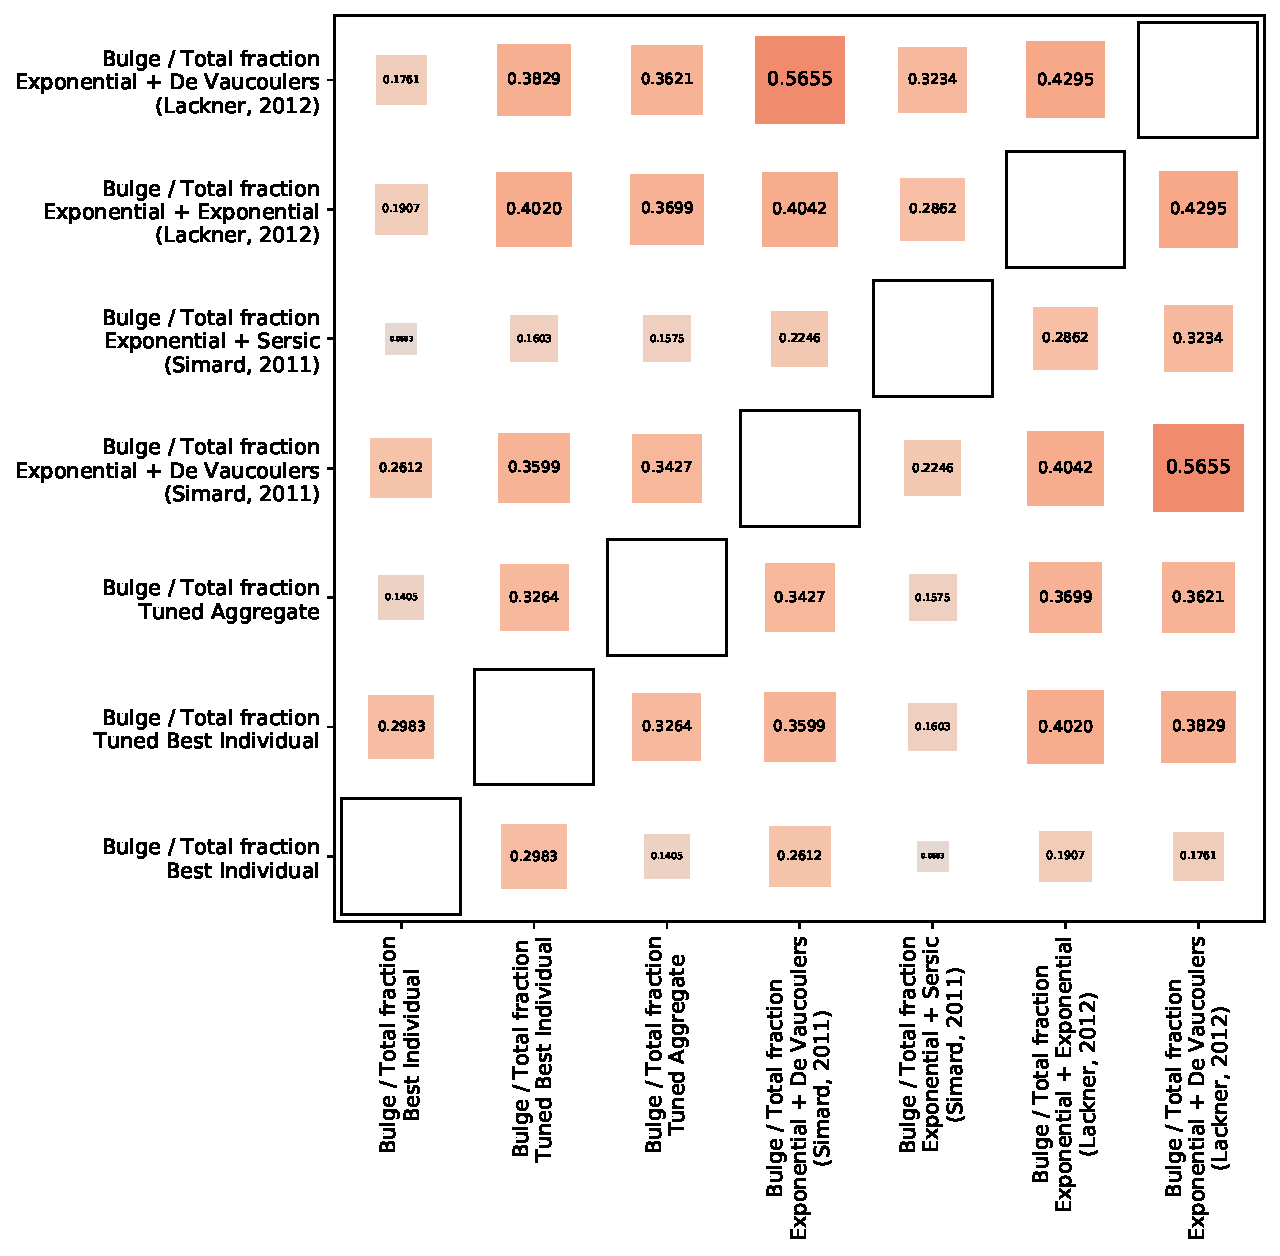
\includegraphics[width=17cm]{images__results/b-t_comparison_correlation.pdf}
  \caption{Correlation matrix showing Kendall rank correlation coefficient between measures of Bulge to Total fraction from \textit{Galaxy Builder} results and other models fitted in \citet{2011ApJS..196...11S} and \citet{2012MNRAS.421.2277L}. Colours and box size indicate the strength of the correlation.}
  \label{fig:bt_correlation}
\end{figure*}


\subsubsection{Comparison to Disc-Bulge-Bar models}

\citet{2018MNRAS.473.4731K} performed multi-component, multi-band decompositions of a selection of SDSS galaxies, 12 of which were also classified in \textit{Galaxy Builder}. Figure \ref{fig:sd_comp_comparison} compares the axis ratios and effective radii of bulges, discs and bars in \citet{2018MNRAS.473.4731K} to those present in the aggregate models. We see strong agreement in disk effective radius and axis ratio, with significantly more scatter in the sizes and shapes of the central components. We hypothesize that this is caused by difficult parameter degeneracies and issues with tuning, as the aggregate model without tuning shows closer agreeement (with systematic errors in size due to the nature of the clustering).

\begin{figure}
  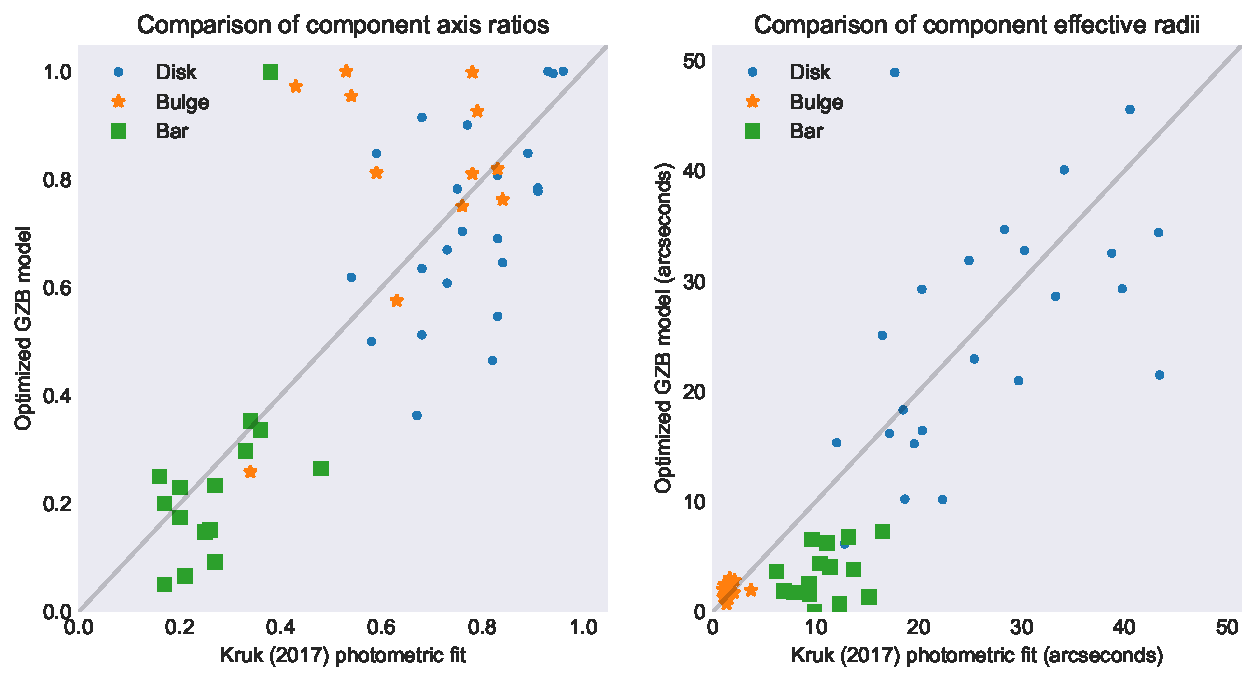
\includegraphics[width=8cm]{images__results/sd_comp_comparison.pdf}
  \caption{Comparison between \textit{Galaxy Builder} aggregate models (without fitting) and the result of 3-component, multi\-wavelength fits performed by \citet{2018MNRAS.473.4731K}. Discs, Bulges and Bars are shown as blue circles, orange stars and green squares respectively. The left panel compares component effective radius, the right panel compares the component axis ratio.}
  \label{fig:sd_comp_comparison}
\end{figure}


\subsubsection{Comparison to Disc-Bulge-Bar-Spiral models}
To the best of our knowledge, no photometic models exist for the Galaxy Builder sample which contain spiral arm structure. The closest comparable result is that produced by \citet{Gao2017:1709.00746v1}, however the galaxies they used are not in the Sloan footprint.

In order to provide a comparison for our novel method of spiral parameter (pitch angle and amplitude) extraction, we compare the result of our logarithmic spiral fit to the relationship obtained by \citet{Hart2016:1607.01019v1} between GZ2 classification and galaxy pitch angle (Figure \ref{fig:hart_pitch_angle}). Their fit was obtained by using the Zooniverse to filter good vs bad spiral arm segments identified using a leading automated spiral arm detection and fitting tool, \textsc{SpArcFiRe} \citep{Davis2014:1402.1910v1}, whereas \textit{Galaxy Builder} asks volunteers to provide their own opinion on spiral arm number, location and tightness. \textit{Galaxy Builder} pitch angles are within the uncertainties on the \citet{Hart2016:1607.01019v1} fit, even when not accounting for error on our measurements.

Many researches (\citealt{Davis2014:1402.1910v1}, \citealt{2019arXiv190804246D} to name a few) have noted that many galaxies show large inter-arm variations in pitch angle, suggesting that obtaining a single value of a galaxy's pitch angle is highly dependent on which arms have been identified. We plan to further explore this issue in a future work.

\begin{figure}
  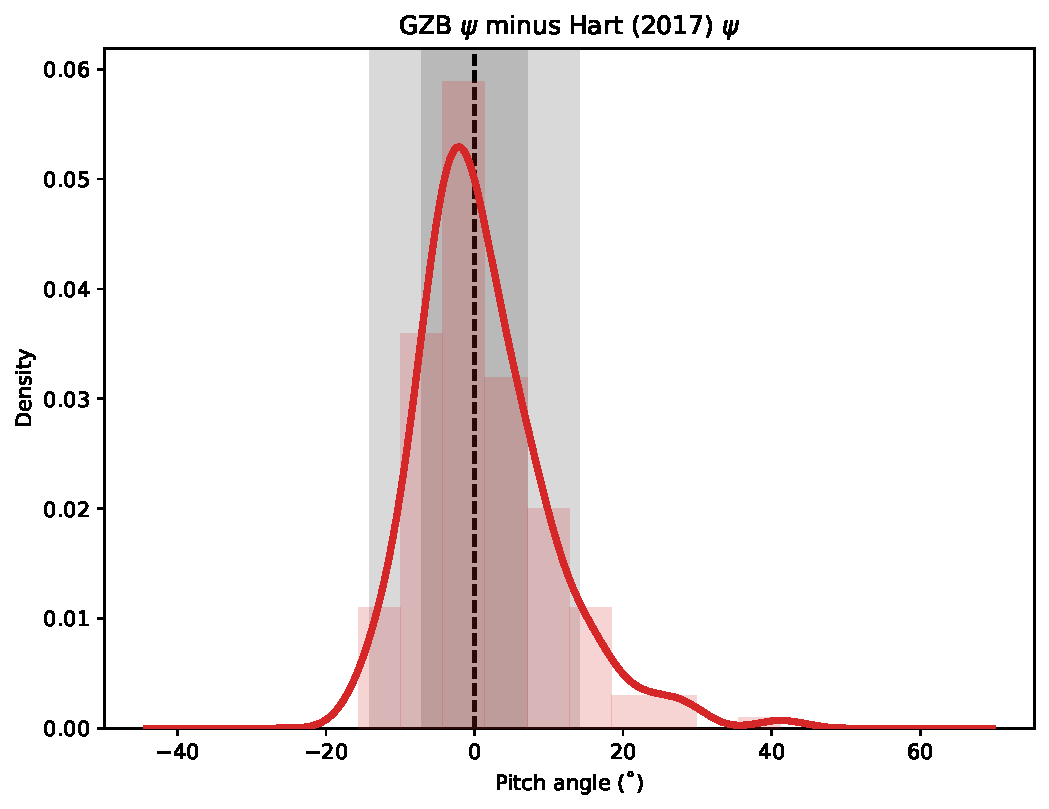
\includegraphics[width=8cm]{images__results/gzb-hart-comparison.pdf}
  \caption{A comparison of Pitch angle obtained by \citet{Hart2016:1607.01019v1} with measured pitch angles for the aggregated model results in galaxies in the Galaxy Zoo Builder sample. The grey regions show 1- and $2\sigma$ errors from \citet{Hart2016:1607.01019v1}. Errors on \textit{Galaxy Builder}-measured pitch angles are not accounted for.}
  \label{fig:hart_pitch_angle}
\end{figure}

\end{document}
